\documentclass{beamer}
\usepackage{amsfonts,amsmath,oldgerm}
\usetheme{sintef}
\usepackage{xeCJK}
\newcommand{\testcolor}[1]{\colorbox{#1}{\textcolor{#1}{test}}~\texttt{#1}}
\usefonttheme[onlymath]{serif}
\titlebackground*{figures/background}
\newcommand{\hrefcol}[2]{\textcolor{cyan}{\href{#1}{#2}}}

% Page 1

\title{从零开始的Cocos2d-x开发指南}
\subtitle{Starting from Scratch: A Cocos2d-x Development Guide}
\course{计算机科学与技术学院}
\author{林继申}
\IDnumber{2250758}
\date{2024年12月1日}

\begin{document}
\maketitle

% Page 2

\begin{frame}[fragile]{LaTeX Beamer Template}
\framesubtitle{Acknowledgements}
本演示文稿由同济大学演示文稿模板(Tongji University Beamer Template)编译。

\vspace{1em}

\hrefcol{https://github.com/MinmusLin/Tongji_University_Beamer_Template}{GitHub仓库}

\vspace{1em}

特别感谢 Federico Zenith 提供的 SINTEF Presentation 模板,以及 Liu Qilong 开发的 Beamer-LaTeX-Themes 派生版本。同时,也感谢 wzl-plasmid 对模板样式的贡献。本项目在这些优秀作品的基础上进行了改进,感谢开源社区所有开发者的支持与贡献。
\end{frame}

% Page 3

\section{Cocos2d-x简介}

% Page 4

\begin{chapter}[figures/background_negative]{}{Cocos2d-x简介}
\framesubtitle{Introduction to Cocos2d-x}
\begin{itemize}
\item Cocos产品
\begin{itemize}
\item Cocos Creator
\item Cocos2d-x
\item Cocos Runtime
\end{itemize}
\item 为什么推荐Cocos2d-x
\item 如何上手Cocos2d-x引擎
\end{itemize}
\end{chapter}

% Page 5

\begin{frame}[fragile]{Cocos产品}
Cocos是一个开源的游戏开发引擎,提供强大的工具和框架,用于创建跨平台的2D和3D游戏,支持C++、JavaScript 和Lua等多种编程语言。
\begin{itemize}
\item \textbf{Cocos Creator}:一款高效、轻量开源的跨平台图形引擎,也是一个实时3D内容创作平台。
\item \textbf{Cocos2d-x}:一个高性能的C++、Lua、JavaScript游戏引擎,跨平台支持iOS、Android等智能手机,Windows、Mac等桌面操作系统,以及Chrome、Safari、IE等HTML5浏览器。
\item \textbf{Cocos Runtime}:一个支持互动内容免安装即可运行的商业化SDK,支持主流JavaScript游戏引擎开发的内容,为用户提供数字互动内容“点开即玩”的畅爽体验。
\end{itemize}
\end{frame}

% Page 6

\begin{frame}[fragile]{Cocos Creator}
Cocos Creator:开源、高效、性能卓越的跨平台3D实时内容创作引擎。

\vspace{1em}

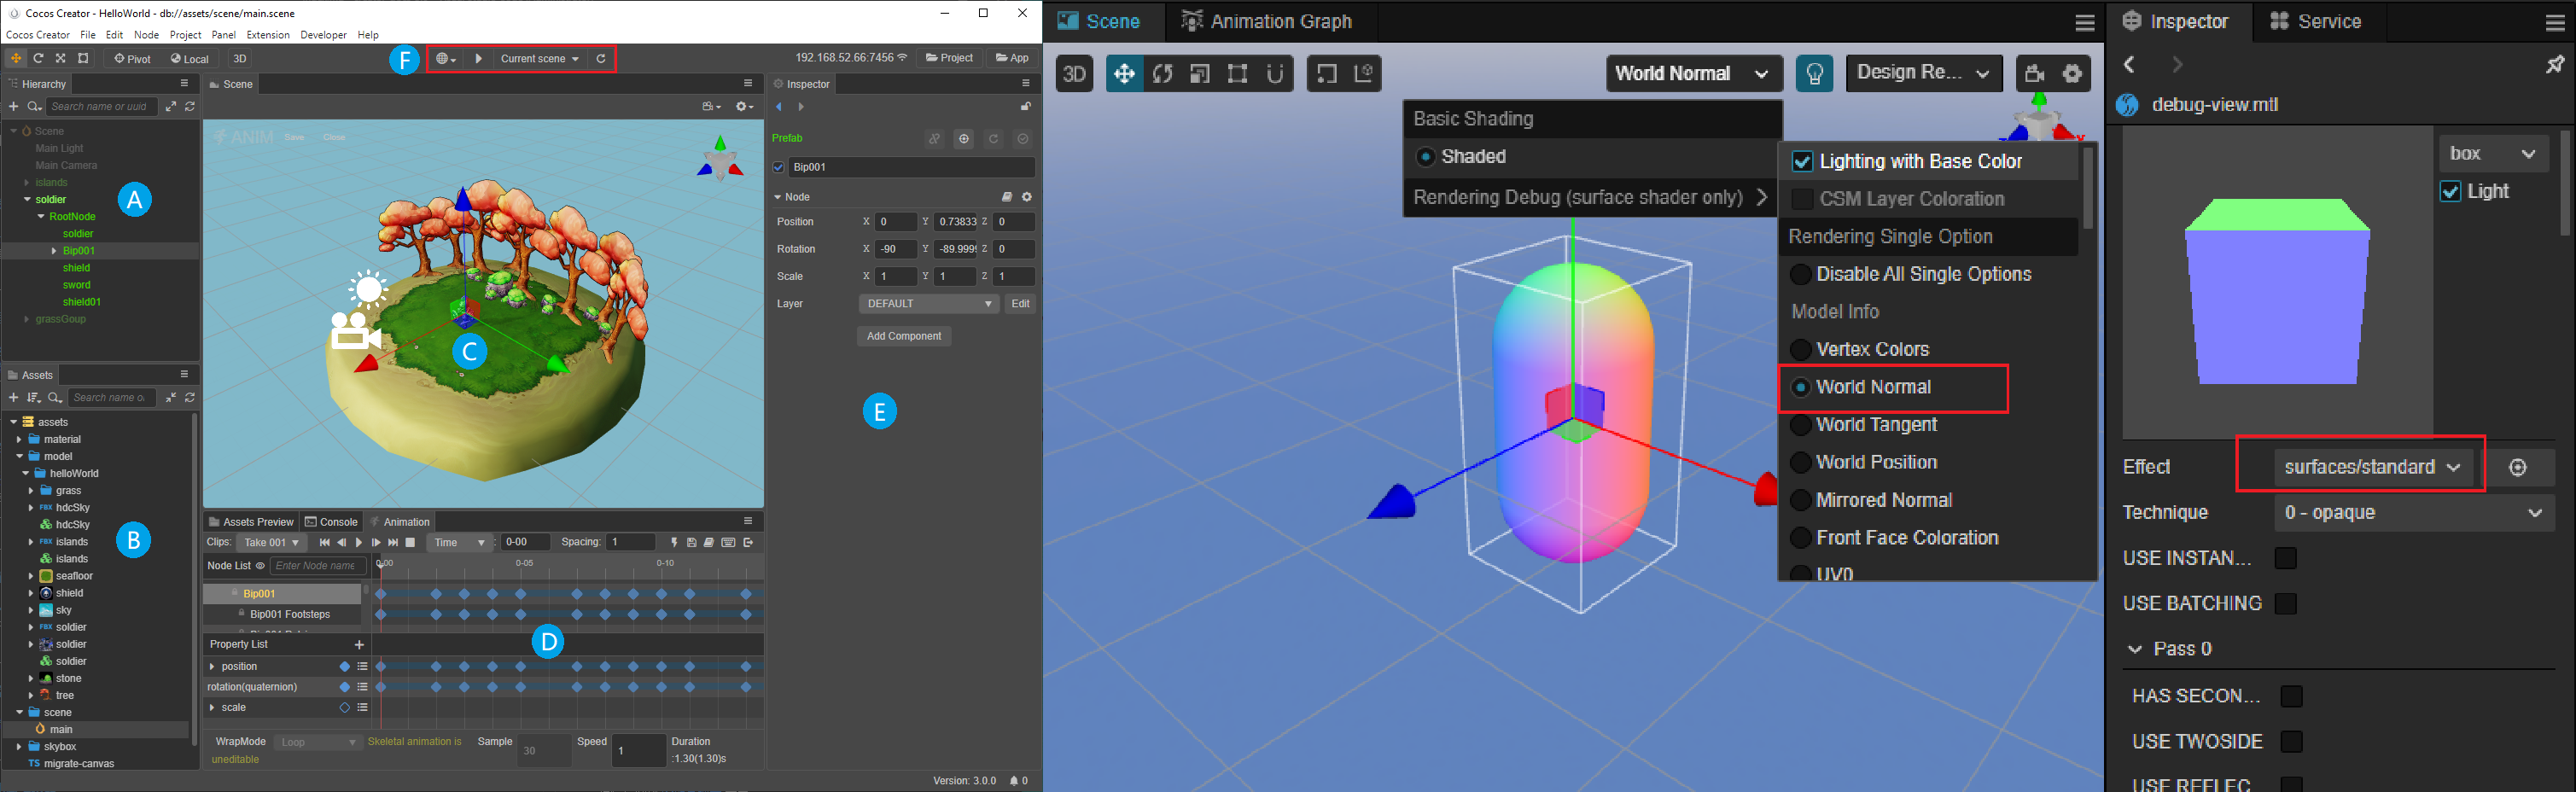
\includegraphics[width=\textwidth]
{figures/cocos_creator}

\vspace{1em}

(\hrefcol{https://docs.cocos.com/creator/3.8/manual/zh}{Cocos Creator 3.8用户手册}、\hrefcol{https://dev.epicgames.com/documentation/zh-cn/unreal-engine/unreal-engine-5-5-documentation}{虚幻引擎5.5文档})
\end{frame}

% Page 7

\begin{frame}[fragile]{Cocos2d-x}
\begin{columns}
\begin{column}{0.5\textwidth}
Cocos2d-x:开源、开放、灵活、轻量,即刻帮你拓展边界。

\vspace{1em}

Cocos2d-x在2019年停止更新。

\vspace{1em}

Cocos2d-x市场占有情况:使用Cocos2d-x开发的许多游戏占据苹果应用商店和谷歌应用商店排行榜,同时许多公司如触控、谷歌、微软、ARM,英特尔及的黑莓工程师在Cocos2d-x领域也非常活跃。
\end{column}
\begin{column}{0.5\textwidth}
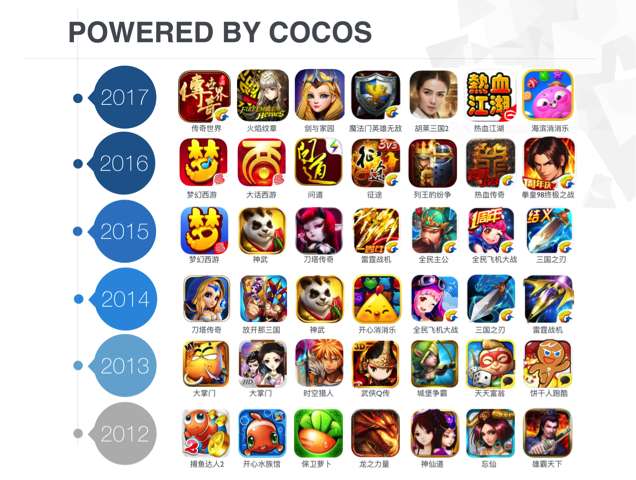
\includegraphics[width=\textwidth]
{figures/cocos2dx_games}
\end{column}
\end{columns}
\end{frame}

% Page 8

\begin{frame}[fragile]{Cocos2d-x}
\begin{columns}
\begin{column}{0.7\textwidth}
Cocos官网提供了如下学习资源和参考资料:
\begin{itemize}
\item \hrefcol{https://docs.cocos.com/cocos2d-x/manual/zh}{Cocos2d-x官方文档}
\item \hrefcol{https://docs.cocos2d-x.org/api-ref}{Cocos2d-x API文档}
\item \hrefcol{https://github.com/cocos2d/cocos2d-x}{Cocos2d-x源代码}
\item \hrefcol{https://github.com/cocos2d/cocos2d-x/tree/v3/tests}{Cocos2d-x引擎官方测试项目}
\item \hrefcol{https://github.com/cocos2d/cocos2d-x-samples}{Cocos2d-x示例程序}
\end{itemize}

\vspace{1em}

Cocos2d-x官方文档是最好的入门学习资源,没有之一。

ChatGPT是最好的Debug工具,没有之一。(:D)
\end{column}
\begin{column}{0.3\textwidth}

\includegraphics[width=\textwidth]
{figures/cocos2dx}
\end{column}
\end{columns}
\end{frame}

% Page 9

\section{Cocos2d-x基本概念}

% Page 10

\begin{chapter}[figures/background_negative]{}{Cocos2d-x基本概念}
\framesubtitle{Basic Concepts of Cocos2d-x}
\begin{itemize}
\item 游戏引擎与组件
\begin{itemize}
\item 导演 - 单例模式
\item 场景 - 场景图
\item 精灵
\item 动作与序列
\end{itemize}
\item 节点关系
\item 日志输出
\end{itemize}
\end{chapter}

% Page 11

\begin{frame}[fragile]{游戏引擎}
游戏引擎是一种特殊的软件,它提供游戏开发时需要的常见功能;引擎会提供许多组件,使用这些组件能缩短开发时间,让游戏开发变得更简单。

\vspace{1em}

Cocos2d-x提供了许多易于使用的组件,有着更好的性能,还同时支持移动端和桌面端。Cocos2d-x通过封装底层图形接口提供了易用的API,降低了游戏开发的门槛,让使用者可以专注于开发游戏,而不用关注底层的技术细节。(\hrefcol{https://github.com/MinmusLin/Advanced_Language_Programming_and_OOP_Course_Projects/blob/main/common/FastPrinter.cpp}{FastPrinter.cpp}、\hrefcol{https://github.com/MinmusLin/Advanced_Language_Programming_and_OOP_Course_Projects/blob/main/common/lib_hdc_tools.cpp}{lib\_hdc\_tools.cpp})

\vspace{1em}

更重要的是Cocos2d-x是一个完全开源的游戏引擎,这就允许您在游戏开发过程中根据实际需要,定制化引擎的功能。(\hrefcol{https://github.com/MinmusLin/Teamfight_Tactics/blob/main/Classes/Button}{HoverButton类})
\end{frame}

% Page 12

\begin{frame}[fragile]{组件}
游戏界面由组件构成。

\vspace{1em}

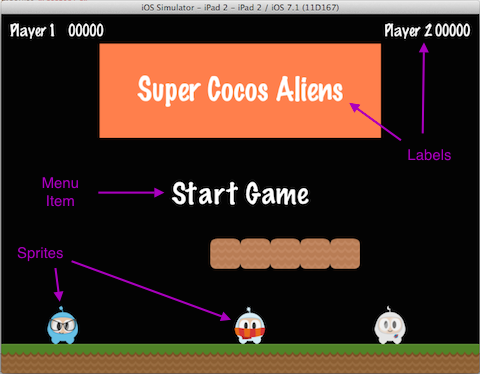
\includegraphics[width=0.5\textwidth]
{figures/components}
\end{frame}

% Page 13

\begin{frame}[fragile]{导演(Director)}
Cocos2d-x使用导演的概念。在使用Cocos2d-x开发游戏的过程中,你可以认为自己是执行制片人,告诉导演该怎么办!一个常见的Director任务是控制场景替换和转换。Director是一个共享的\textbf{单例对象},可以在代码中的任何地方调用。

\vspace{1em}

这是一个典型的游戏流程实例。当您的游戏设计好时,Director就负责场景的转换:

\vspace{1em}

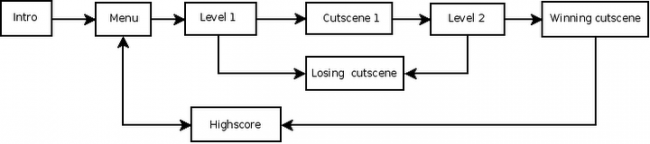
\includegraphics[width=\textwidth]
{figures/director}
\end{frame}

% Page 14

\begin{frame}[fragile]{单例模式(Singleton Pattern)}
单例模式(Singleton Pattern)是一种设计模式,它的主要目的是确保一个类只有一个实例,并提供一个全局访问点来获取该实例。这样可以保证在整个程序运行期间,某个类的实例不会被多次创建,从而节省系统资源并确保一致性。(\hrefcol{https://github.com/MinmusLin/Teamfight_Tactics/tree/main/Classes/LocationMap}{LocationMap类})

\vspace{1em}

单例模式的核心要点:
\begin{itemize}
\item \textbf{类的构造函数是私有的}:避免外部代码通过构造函数直接创建多个实例。
\item \textbf{静态成员变量}:存储唯一的实例。
\item \textbf{静态成员函数}:提供对外的访问接口,用于获取唯一的实例。
\end{itemize}
\end{frame}

% Page 15

\begin{frame}[fragile]{场景(Scene)}
在游戏开发过程中,你可能需要一个主菜单,几个关卡和一个结束场景。如何组织所有这些分开的部分?使用场景(Scene)!(\hrefcol{https://github.com/MinmusLin/Teamfight_Tactics/tree/main/Classes/Scene}{Scene类})

\vspace{1em}

场景是由很多小的对象拼接而成,所有的对象组合在一起,形成了最终的结果。场景是被\textbf{渲染器(renderer)}画出来的。渲染器负责渲染精灵和其它的对象进入屏幕。为了更好的理解这个过程,我们需要讨论一下\textbf{场景图}。
\end{frame}

% Page 16

\begin{frame}[fragile]{场景图(Scene Graph)}
\begin{columns}
\begin{column}{0.65\textwidth}
场景图(Scene Graph)是一种安排场景内对象的数据结构,它把场景内所有的节点(Node)都包含在一个树(Tree)上。(场景图虽然叫做“图”,但实际使用一个树结构来表示)。

\vspace{1em}

当你开发游戏的时候,你会添加一些节点,精灵和动画到一个场景中,你期望的是每一个添加的对象都能被正确的展示,可是如果有个对象没有被展示呢?可能你错误的把这个对象隐藏到背景中了。

\vspace{1em}

既然场景图是一个树结构,你就能遍历它,Cocos2d-x使用中序遍历,先遍历左子树,然后根节点,最后是右子树。中序遍历下图的节点,能得到A, B, C, D, E, F, G, H, I这样的序列。
\end{column}
\begin{column}{0.35\textwidth}
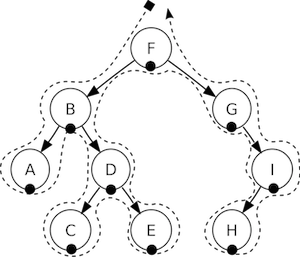
\includegraphics[width=\textwidth]
{figures/scene_graph}
\end{column}
\end{columns}
\end{frame}

% Page 17

\begin{frame}[fragile]{场景图(Scene Graph)}
在Cocos2d-x中,通过Scene的\texttt{addChild()}方法构建场景图。

\vspace{1em}

渲染时z-order值大的节点对象会后绘制,值小的节点对象先绘制。如果两个节点对象的绘制范围有重叠,z-order值大的可能会覆盖z-order值小的。

\begin{block}{添加场景}
\begin{verbatim}
scene->addChild(title_node, -2);

scene->addChild(label_node);

scene->addChild(sprite_node, 1);
\end{verbatim}
\end{block}
\end{frame}

% Page 18

\begin{frame}[fragile]{精灵(Sprite)}
精灵是能在屏幕上移动的对象,它能被控制。

\vspace{1em}

每个图形对象都是一个精灵吗?不是的。为什么? 如果你能控制它,它才是一个精灵,如果无法控制,那就只是一个节点(Node)。

\vspace{1em}

Sprite很容易被创建,它有一些可以被配置的属性,比如:位置,旋转角度,缩放比例,透明度,颜色等等。
\end{frame}

% Page 19

\begin{frame}[fragile]{精灵(Sprite)}
\begin{block}{配置位置、旋转角度、缩放比例}
\begin{verbatim}
auto mySprite = Sprite::create("mysprite.png");
mySprite->setPosition(Vec2(500, 0));
mySprite->setRotation(40);
mySprite->setScale(2.0);
\end{verbatim}
\end{block}
\begin{columns}
\begin{column}{0.3\textwidth}
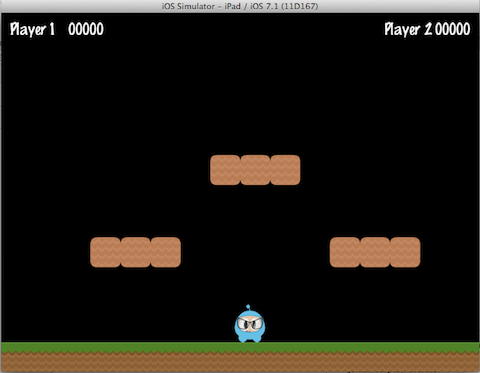
\includegraphics[width=\textwidth]
{figures/set_position}
\end{column}
\begin{column}{0.3\textwidth}
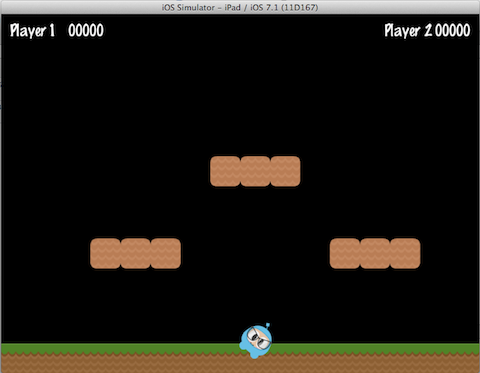
\includegraphics[width=\textwidth]
{figures/set_rotation}
\end{column}
\begin{column}{0.3\textwidth}
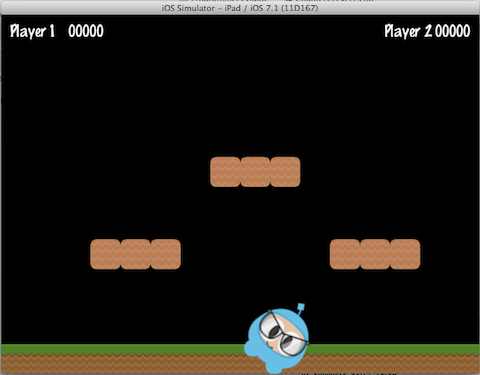
\includegraphics[width=\textwidth]
{figures/set_scale}
\end{column}
\end{columns}
\end{frame}

% Page 20

\begin{frame}[fragile]{精灵(Sprite)}
\begin{block}{配置锚点}
\begin{verbatim}
mySprite->setAnchorPoint(Vec2(0, 0));
mySprite->setAnchorPoint(Vec2(0.5, 0.5));
mySprite->setAnchorPoint(Vec2(1, 1));
\end{verbatim}
\end{block}
\begin{columns}
\begin{column}{0.3\textwidth}
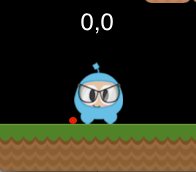
\includegraphics[width=\textwidth]
{figures/set_anchor_point_1}
\end{column}
\begin{column}{0.3\textwidth}
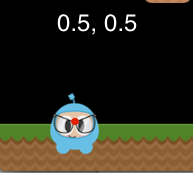
\includegraphics[width=\textwidth]
{figures/set_anchor_point_2}
\end{column}
\begin{column}{0.3\textwidth}
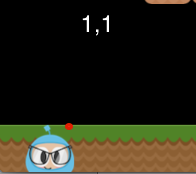
\includegraphics[width=\textwidth]
{figures/set_anchor_point_3}
\end{column}
\end{columns}
\end{frame}

% Page 21

\begin{frame}[fragile]{动作(Action)}
动作(Action)可以让精灵在场景中移动,如从一个点移动到另外一个点。
\begin{block}{执行动作}
\begin{verbatim}
auto mySprite = Sprite::create("mysprite.png");

// 创建 MoveBy,让精灵在 2 秒内向右移动 50 像素,向上移动 10 像素
auto moveBy = MoveBy::create(2, Vec2(50,10));
mySprite->runAction(moveBy);

// 创建 MoveTo,让精灵在 2 秒内移动到指定位置 (50, 10)
auto moveTo = MoveTo::create(2, Vec2(50,10));
mySprite->runAction(moveTo);
\end{verbatim}
\end{block}
\end{frame}

% Page 22

\begin{frame}[fragile]{序列(Sequence)}
序列(Sequence)支持执行多个Action。
\begin{block}{执行动作序列}
\begin{verbatim}
auto mySprite = Node::create();

auto moveTo1 = MoveTo::create(2, Vec2(50,10));
auto moveBy1 = MoveBy::create(2, Vec2(100,10));
auto moveTo2 = MoveTo::create(2, Vec2(150,10));
auto delay = DelayTime::create(1);

mySprite->runAction(Sequence::create(moveTo1, delay, moveBy1,
                    delay.clone(), moveTo2, nullptr));
\end{verbatim}
\end{block}
\end{frame}

% Page 23

\begin{frame}[fragile]{序列(Sequence)}
通过引擎中的Spawn对象,能让多个动作同时被解析执行。可能不同动作的执行时间不一致,在这种情况下,他们不会同时结束。
\begin{block}{同时执行多个动作}
\begin{verbatim}
auto myNode = Node::create();

auto moveTo1 = MoveTo::create(2, Vec2(50,10));
auto moveBy1 = MoveBy::create(2, Vec2(100,10));
auto moveTo2 = MoveTo::create(2, Vec2(150,10));

myNode->runAction(Spawn::create(moveTo1, moveBy1, moveTo2, nullptr));
\end{verbatim}
\end{block}
\end{frame}

% Page 24

\begin{frame}[fragile]{节点关系}
Cocos2d-x的节点关系,是被附属和附属的关系,就像数据结构中的父子关系,如果两个节点被添加到一个父子关系中,那么父节点的属性变化会被自动应用到子节点中。

\vspace{1em}

需要注意的是,父节点的属性(如位置、缩放、旋转等)会影响到子节点的变换效果(例如子节点的位置、大小和旋转角度等),但是父节点的锚点不会直接改变子节点的锚点。子节点的锚点总是相对于子节点自身的坐标系独立存在,不会被父节点的锚点所影响。父节点的锚点变动会影响子节点在父节点坐标系中的位置变换,但不会影响子节点本身的锚点。
\end{frame}

% Page 25

\begin{frame}[fragile]{日志输出}
有时,在你的游戏正在运行的时候,为了了解程序的运行过程或是为了查找一个Bug,你想看到一些运行时信息,可以使用\texttt{log()}把信息输出到控制台。

\vspace{1em}

\begin{block}{日志输出}
\begin{verbatim}
log("This would be outputted to the console");
log("string is %s", s);
log("double is %f", d);
log("integer is %d", i);
log("float is %f", f);
\end{verbatim}
\end{block}

\vspace{1em}

对于使用C++进行游戏开发的用户来说,可能想使用\texttt{std::cout}而不用\texttt{log()},实际上\texttt{log()}更易于使用,它格式化复杂的输出信息更简单。
\end{frame}

% Page 26

\section{Cocos2d-x基本功能}

% Page 27

\begin{chapter}[figures/background_negative]{}{Cocos2d-x基本功能}
\framesubtitle{Basic Features of Cocos2d-x}
\begin{itemize}
\item 基本功能
\begin{itemize}
\item 精灵 - Sprite类方法
\item 动作 - 动作序列分析
\item 场景 - 场景创建与场景切换
\end{itemize}
\item 如何查阅官方文档
\end{itemize}
\end{chapter}

% Page 28

\begin{frame}[fragile]{精灵(Sprite)}
在\hrefcol{https://docs.cocos.com/cocos2d-x/manual/zh/sprites}{Cocos2d-x官方文档}中,关于精灵部分给出了以下内容:
\begin{itemize}
\item \textbf{精灵创建}:使用图像创建、使用图集创建、使用精灵缓存创建
\item \textbf{精灵控制}:锚点、位置、旋转、缩放、倾斜、颜色、透明度
\item \textbf{多边形精灵}:为什么要使用多边形精灵、AutoPolygon
\end{itemize}

\vspace{1em}

阅读官方文档是程序开发者的必备能力。

\vspace{1em}

完整精灵(Sprite)类方法在\hrefcol{https://docs.cocos2d-x.org/api-ref/cplusplus/v4x/d3/d5c/classcocos2d_1_1_sprite.html}{Cocos2d-x API文档}中获取。
\end{frame}

% Page 29

\begin{frame}[fragile]{精灵(Sprite)类方法}
公共成员函数:
\begin{itemize}
\item \texttt{virtual bool isFrameDisplayed (SpriteFrame *frame) const}

返回一个布尔值,表示当前是否正在显示指定的 \texttt{SpriteFrame}
\item \texttt{virtual SpriteFrame *getSpriteFrame () const}

返回当前显示的帧
\item \texttt{V3F\_C4B\_T2F\_Quad getQuad () const}

返回精灵的四边形(纹理坐标、顶点坐标和颜色)信息
\item \texttt{bool isTextureRectRotated () const}

返回一个布尔值,表示纹理矩形是否被旋转
\item \texttt{unsigned int getAtlasIndex () const}

返回在纹理图集中的索引
\item \texttt{void setAtlasIndex (unsigned int atlasIndex)}

设置纹理图集的索引
\end{itemize}
\end{frame}

% Page 30

\begin{frame}[fragile]{精灵(Sprite)类方法}
公共成员函数:
\begin{itemize}
\item \texttt{const Rect \&getTextureRect () const}

返回精灵的纹理矩形
\item \texttt{TextureAtlas *getTextureAtlas () const}

获取精灵渲染时所使用的纹理图集的弱引用
\item \texttt{virtual void setProgramState (backend::ProgramState *programState) override}

设置程序状态
\item \texttt{virtual backend::ProgramState *getProgramState () const override}

获取当前的程序状态
\item \texttt{void setTextureAtlas (TextureAtlas *textureAtlas)}

设置精灵渲染时使用的纹理图集的弱引用
\item \texttt{const Vec2 \&getOffsetPosition () const}

获取精灵的偏移位置
\end{itemize}
\end{frame}

% Page 31

\begin{frame}[fragile]{精灵(Sprite)类方法}
公共成员函数:
\begin{itemize}
\item \texttt{bool isFlippedX () const}

返回一个布尔值,表示精灵是否水平翻转
\item \texttt{void setFlippedX (bool flippedX)}

设置精灵是否水平翻转
\item \texttt{bool isFlippedY () const}

返回一个布尔值,表示精灵是否垂直翻转
\item \texttt{void setFlippedY (bool flippedY)}

设置精灵是否垂直翻转
\item \texttt{const PolygonInfo \&getPolygonInfo () const}

返回与精灵关联的多边形信息的引用
\item \texttt{void setPolygonInfo (const PolygonInfo \&info)}

设置精灵使用的新多边形信息
\end{itemize}
\end{frame}

% Page 32

\begin{frame}[fragile]{精灵(Sprite)类方法}
公共成员函数:
\begin{itemize}
\item \texttt{void setStretchEnabled (bool enabled)}

设置是否启用内容大小拉伸纹理
\item \texttt{bool isStretchEnabled () const}

返回一个布尔值,表示内容大小是否拉伸纹理
\end{itemize}
批处理节点方法:
\begin{itemize}
\item \texttt{virtual void updateTransform () override}

根据旋转、位置和缩放值更新四边形
\item \texttt{virtual SpriteBatchNode *getBatchNode () const}

返回精灵渲染时使用的批处理节点对象
\item \texttt{virtual void setBatchNode (SpriteBatchNode *spriteBatchNode)}

设置批处理节点
\end{itemize}
\end{frame}

% Page 33

\begin{frame}[fragile]{精灵(Sprite)类方法}
纹理 / 帧方法:
\begin{itemize}
\item \texttt{virtual void setTexture (const std::string \&filename)}

设置一个新的纹理(通过文件名)
\item \texttt{virtual void setTexture (Texture2D *texture) override}

设置新的纹理(通过 \texttt{Texture2D} 对象),并且纹理的矩形不会改变
\item \texttt{virtual Texture2D *getTexture () const override}

返回精灵使用的 \texttt{Texture2D} 对象
\item \texttt{virtual void setTextureRect (const Rect \&rect)}

更新精灵的纹理矩形
\item \texttt{virtual void setTextureRect (const Rect \&rect, bool rotated, const Size \&untrimmedSize)}

通过不同的参数更新纹理矩形,包括是否旋转和未裁剪的尺寸
\item \texttt{virtual void setVertexRect (const Rect \&rect)}

设置顶点矩形
\end{itemize}
\end{frame}

% Page 34

\begin{frame}[fragile]{精灵(Sprite)类方法}
纹理 / 帧方法:
\begin{itemize}
\item \texttt{virtual void setCenterRectNormalized (const Rect \&rect)}

设置规范化的中心矩形
\item \texttt{virtual Rect getCenterRectNormalized () const}

获取规范化的中心矩形
\item \texttt{virtual void setCenterRect (const Rect \&rect)}

设置中心矩形
\item \texttt{virtual Rect getCenterRect () const}

返回 Cap Insets 矩形
\item \texttt{virtual void setSpriteFrame (const std::string \&spriteFrameName)}

设置精灵帧(通过名称)
\item \texttt{virtual void setSpriteFrame (SpriteFrame *newFrame)}

设置精灵帧(通过 \texttt{SpriteFrame} 对象)
\end{itemize}
\end{frame}

% Page 35

\begin{frame}[fragile]{精灵(Sprite)类方法}
动画方法:
\begin{itemize}
\item \texttt{virtual void setDisplayFrameWithAnimationName (const std::string \&animationName, unsigned int frameIndex)}

根据动画名称和帧索引设置当前显示的帧
\end{itemize}
精灵属性的设置器 / 获取器:
\begin{itemize}
\item \texttt{virtual bool isDirty () const}

返回一个布尔值,表示精灵是否需要在图集中更新
\item \texttt{virtual void setDirty (bool dirty)}

设置精灵为脏状态,表示需要在图集中更新
\item \texttt{virtual std::string getDescription () const override}

获取精灵的描述信息
\end{itemize}
\end{frame}

% Page 36

\begin{frame}[fragile]{精灵(Sprite)类方法}
从Node类继承的函数:
\begin{itemize}
\item \texttt{virtual void setScaleX (float scaleX) override}

设置节点的水平缩放
\item \texttt{virtual void setScaleY (float scaleY) override}

设置节点的垂直缩放
\item \texttt{virtual void setScale (float scaleX, float scaleY) override}

设置节点的水平和垂直缩放
\item \texttt{virtual void setPosition (const Vec2 \&pos) override}

设置节点在父节点坐标系统中的位置
\item \texttt{virtual void setPosition (float x, float y) override}

设置节点在父节点坐标系统中的位置
\item \texttt{virtual void setRotation (float rotation) override}

设置节点的旋转角度(以度为单位)
\end{itemize}
\end{frame}

% Page 37

\begin{frame}[fragile]{精灵(Sprite)类方法}
从Node类继承的函数:
\begin{itemize}
\item \texttt{virtual void setRotationSkewX (float rotationX) override}

设置节点的水平旋转(以度为单位)
\item \texttt{virtual void setRotationSkewY (float rotationY) override}

设置节点的垂直旋转(以度为单位)
\item \texttt{virtual void setSkewX (float sx) override}

设置节点的水平倾斜角度(以度为单位)
\item \texttt{virtual void setSkewY (float sy) override}

设置节点的垂直倾斜角度(以度为单位)
\item \texttt{virtual void removeChild (Node *child, bool cleanup) override}

从容器中移除子节点
\item \texttt{virtual void removeAllChildrenWithCleanup (bool cleanup) override}

移除容器中的所有子节点,并根据 \texttt{cleanup} 参数进行清理
\end{itemize}
\end{frame}

% Page 38

\begin{frame}[fragile]{精灵(Sprite)类方法}
从Node类继承的函数:
\begin{itemize}
\item \texttt{virtual void reorderChild (Node *child, int zOrder) override}

根据新的 z 值重新排序子节点
\item \texttt{virtual void addChild (Node *child, int zOrder, int tag) override}

将子节点添加到容器中,并指定 z 顺序和标签
\item \texttt{virtual void addChild (Node *child, int zOrder, const std::string \&name) override}

将子节点添加到容器中,并指定 z 顺序和名称
\item \texttt{virtual void sortAllChildren () override}

在绘制之前对子节点进行排序
\item \texttt{virtual void setScale (float scale) override}

设置节点的缩放
\item \texttt{virtual void setPositionZ (float positionZ) override}

设置节点的 Z 坐标
\end{itemize}
\end{frame}

% Page 39

\begin{frame}[fragile]{精灵(Sprite)类方法}
从Node类继承的函数:
\begin{itemize}
\item \texttt{virtual void setAnchorPoint (const Vec2 \&anchor) override}

设置节点的锚点(以百分比表示)
\item \texttt{virtual void setContentSize (const Size \&size) override}

设置节点的原始大小
\item \texttt{virtual void setIgnoreAnchorPointForPosition (bool value) override}

设置是否忽略锚点来定位节点
\item \texttt{virtual void setVisible (bool bVisible) override}

设置节点的可见性
\item \texttt{virtual void draw (Renderer *renderer, const Mat4 \&transform, uint32\_t flags) override}

重写此方法来绘制自定义节点
\end{itemize}
\end{frame}

% Page 40

\begin{frame}[fragile]{精灵(Sprite)类方法}
从Node类继承的函数:
\begin{itemize}
\item \texttt{virtual void setOpacityModifyRGB (bool modify) override}

如果需要透明度影响颜色属性,则设置为 \texttt{true}
\item \texttt{virtual bool isOpacityModifyRGB () const override}

如果透明度会影响 RGB 颜色值,则返回 \texttt{true}
\item \texttt{virtual void addChild (Node *child)}

将子节点添加到容器中,默认 z 顺序为 0
\item \texttt{virtual void addChild (Node *child, int localZOrder)}

将子节点添加到容器中,并指定局部 z 顺序
\item \texttt{virtual void addChild (Node *child, int localZOrder, int tag)}

将子节点添加到容器中,并指定局部 z 顺序和标签
\end{itemize}
\end{frame}

% Page 41

\begin{frame}[fragile]{精灵(Sprite)类方法}
从Node类继承的函数:
\begin{itemize}
\item \texttt{virtual void addChild (Node *child, int localZOrder, const std::string \&name)}

将子节点添加到容器中,并指定局部 z 顺序和名称
\end{itemize}
从TextureProtocol类继承的函数:
\begin{itemize}
\item \texttt{void setBlendFunc (const BlendFunc \&blendFunc) override}

设置混合函数
\item \texttt{onst BlendFunc \&getBlendFunc () const override}

获取混合函数
\end{itemize}
\end{frame}

% Page 42

\begin{frame}[fragile]{精灵(Sprite)类方法}
Creators:
\begin{itemize}
\item \texttt{static Sprite *create ()}

创建一个空的精灵,不带纹理
\item \texttt{static Sprite *create (const std::string \&filename)}

通过图像文件名创建精灵
\item \texttt{static Sprite *create (const PolygonInfo \&info)}

通过多边形信息创建一个多边形精灵
\item \texttt{static Sprite *create (const std::string \&filename, const Rect \&rect)}

通过图像文件名和矩形区域创建精灵
\end{itemize}
\end{frame}

% Page 43

\begin{frame}[fragile]{精灵(Sprite)类方法}
Creators:
\begin{itemize}
\item \texttt{static Sprite *createWithTexture (Texture2D *texture)}

通过 \texttt{Texture2D} 对象创建精灵
\item \texttt{static Sprite *createWithTexture (Texture2D *texture, const Rect \&rect, bool rotated=false)}

通过 \texttt{Texture2D} 对象和矩形区域创建精灵(可选旋转)
\item \texttt{static Sprite *createWithSpriteFrame (SpriteFrame *spriteFrame)}

通过精灵帧创建精灵
\item \texttt{static Sprite *createWithSpriteFrameName (const std::string \&spriteFrameName)}

通过精灵帧名称创建精灵
\end{itemize}
\end{frame}

% Page 44

\begin{frame}[fragile]{查阅官方文档}
\begin{itemize}
\item 官方文档是掌握工具或框架的核心特性和最佳实践
\item 查阅官方文档能够获取最新版本功能、改进和修复
\item 官方文档提供详尽的API、FAQ和代码示例
\item 官方文档避免低效或错误实现
\item 查阅官方文档提高独立问题解决能力
\item 查阅官方文档减少对他人依赖
\item 官方文档统一技术标准,提升团队工作效率
\end{itemize}
\end{frame}

% Page 45

\begin{frame}[fragile]{动作(Actions)}
基本动作:
\begin{itemize}
\item 使用MoveTo和MoveBy完成节点对象在一个设置的时间后移动
\item 使用RotateTo和RotateBy完成节点对象在一个设置的时间后顺时针旋转指定角度
\item 使用ScaleBy和ScaleTo完成节点对象的比例缩放
\item 使用FadeIn和FadeOut完成节点对象的淡入淡出
\item 使用TintTo和TintBy将一个实现了NodeRGB协议的节点对象进行色彩混合
\end{itemize}
\end{frame}

% Page 46

\begin{frame}[fragile]{动作(Actions)}
\begin{columns}
\begin{column}{0.6\textwidth}
变速动作可以让节点对象具有加速度,产生平滑同时相对复杂的动作,所以可以用变速动作来模仿一些物理运动,这样比实际使用物理引擎的性能消耗低,使用起来也简单。当然你也可以将变速动作应用到动画菜单和按钮上,实现你想要的效果。
\end{column}
\begin{column}{0.4\textwidth}
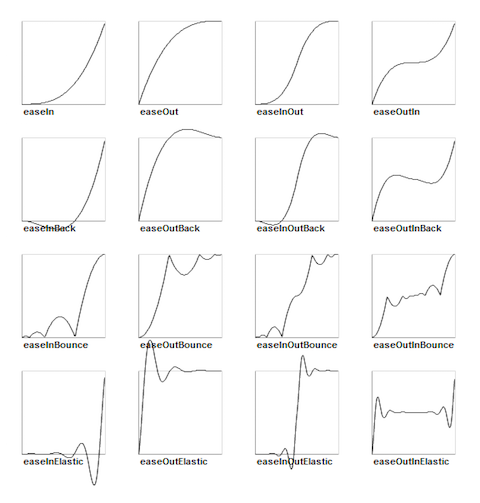
\includegraphics[width=\textwidth]
{figures/variable_speed_motion}
\end{column}
\end{columns}
\end{frame}

% Page 47

\begin{frame}[fragile]{序列(Sequence)}
\begin{columns}
\begin{column}{0.3\textwidth}
动作序列(Sequence)是一种封装多个动作的对象,当这个对象执行时被封装的动作会顺序执行。

\vspace{1em}


\includegraphics[width=\textwidth]
{figures/sequence}
\end{column}
\begin{column}{0.3\textwidth}
Spawn和Sequence是非常相似的,区别是Spawn同时执行所有的动作。

\vspace{1em}

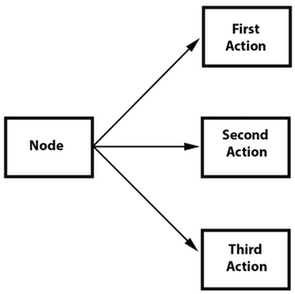
\includegraphics[width=\textwidth]
{figures/spawn}
\end{column}
\begin{column}{0.3\textwidth}
可以把一个Spawn添加到一个Sequence中。

\vspace{1em}

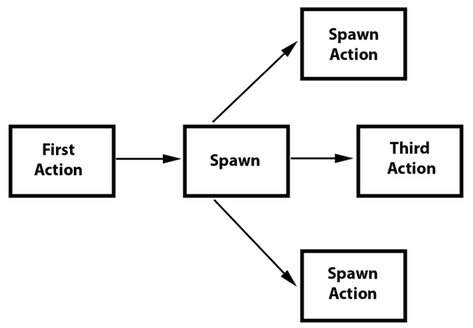
\includegraphics[width=\textwidth]
{figures/spawn_in_sequence}
\end{column}
\end{columns}
\end{frame}

% Page 48

\begin{frame}[fragile]{动作的克隆}
克隆(Clone)的功能和字面含义一样,如果你对一个节点对象使用了\texttt{clone()}方法,你就获得了这个节点对象的拷贝。

\vspace{1em}

为什么要使用\texttt{clone()}方法?因为当Action对象运行时会产生一个内部状态,记录着节点属性的改变。当你想将一个创建的动作,重复使用到不同的节点对象时,如果不用\texttt{clone()}方法,就无法确定这个动作的属性到底是怎样的(因为被使用过,产生了内部状态),这会造成难以预料的结果。
\end{frame}

% Page 49

\begin{frame}[fragile]{动作的克隆}
我们来看示例,假如你有一个坐标位置是 (0,0) 的heroSprite,执行这样一个动作:

\vspace{1em}

\begin{block}{示例动作}
\begin{verbatim}
MoveBy::create(10, Vec2(400,100));
\end{verbatim}
\end{block}

\vspace{1em}

你的 heroSprite 就在 10s 的时间中,从 (0,0) 移动到了 (400,100),heroSprite 有了一个新位置 (400,100),更重要的是动作对象也有了节点位置相关的内部状态了。现在假如你有一个坐标位置是 (200,200) 的 emenySprite。你还使用这个相同的动作,emenySprite 就会移动到 (800,200) 的坐标位置,并不是你期待的结果。因为第二次将这个动作应用的时候,它已经有内部状态了。使用\texttt{clone()}能避免这种情况,克隆获得一个新的动作对象,新的对象没有之前的内部状态。
\end{frame}

% Page 50

\begin{frame}[fragile]{动作的克隆}
\begin{block}{错误示例}
\begin{verbatim}
auto heroSprite = Sprite::create("herosprite.png");
auto enemySprite = Sprite::create("enemysprite.png");

// create an Action
auto moveBy = MoveBy::create(10, Vec2(400,100));

// run it on our hero
heroSprite->runAction(moveBy);

// run it on our enemy
enemySprite->runAction(moveBy); // oops, this will not be unique!
// uses the Actions current internal state as a starting point.
\end{verbatim}
\end{block}
\end{frame}

% Page 51

\begin{frame}[fragile]{动作的克隆}
\begin{block}{正确示例}
\begin{verbatim}
auto heroSprite = Sprite::create("herosprite.png");
auto enemySprite = Sprite::create("enemysprite.png");

// create an Action
auto moveBy = MoveBy::create(10, Vec2(400,100));

// run it on our hero
heroSprite->runAction(moveBy);

// run it on our enemy
enemySprite->runAction(moveBy->clone()); // correct!
// This will be unique.
\end{verbatim}
\end{block}
\end{frame}

% Page 52

\begin{frame}[fragile]{动作的倒转}
倒转(Reverse)的功能也和字面意思一样,调用\texttt{reverse()}可以让一系列动作按相反的方向执行。\texttt{reverse()}不是只能简单的让一个Action对象反向执行,还能让Sequence和Spawn倒转。

\vspace{1em}

\begin{block}{示例动作}
\begin{verbatim}
mySprite->runAction(mySpawn->reverse());
\end{verbatim}
\end{block}
\end{frame}

% Page 53

\begin{frame}[fragile]{动作序列分析}
\begin{block}{动作序列分析}
\begin{verbatim}
auto mySprite = Sprite::create("mysprite.png");
mySprite->setPosition(50, 56);
auto moveBy = MoveBy::create(2.0f, Vec2(500,0));
auto scaleBy = ScaleBy::create(2.0f, 2.0f);
auto delay = DelayTime::create(2.0f);

auto delaySequence = Sequence::create(delay, delay->clone(),
                                      delay->clone(), nullptr);
auto sequence = Sequence::create(moveBy, delay, scaleBy,
                                 delaySequence, nullptr);
mySprite->runAction(sequence);
mySprite->runAction(sequence->reverse());
\end{verbatim}
\end{block}
\end{frame}

% Page 54

\begin{frame}[fragile]{场景创建}
\begin{block}{场景创建}
\begin{verbatim}
auto dirs = Director::getInstance();
Size size = dirs->getVisibleSize();

auto myScene = Scene::create();

auto label1 = Label::createWithTTF("My Game", "Marker Felt.ttf", 36);
label1->setPosition(Vec2(size.width / 2, size.height / 2));
myScene->addChild(label1);

auto sprite1 = Sprite::create("mysprite.png");
sprite1->setPosition(Vec2(100, 100));
myScene->addChild(sprite1);
\end{verbatim}
\end{block}
\end{frame}

% Page 55

\begin{frame}[fragile]{场景切换方式}
\begin{block}{场景切换方式}
\begin{verbatim}
auto myScene = Scene::create();

Director::getInstance()->runWithScene(myScene);
Director::getInstance()->replaceScene(myScene);
Director::getInstance()->pushScene(myScene);
Director::getInstance()->popScene();
\end{verbatim}
\end{block}
\end{frame}

% Page 56

\begin{frame}[fragile]{场景切换方式}
\begin{itemize}
\item \texttt{runWithScene()}用于开始游戏,加载第一个场景。只用于第一个场景!
\item \texttt{replaceScene()}使用传入的场景替换当前场景来切换画面,当前场景被释放。这是切换场景时最常用的方法。
\item \texttt{pushScene()}将当前运行中的场景暂停并压入到场景栈中,再将传入的场景设置为当前运行场景。只有存在正在运行的场景时才能调用该方法。
\item \texttt{popScene()}释放当前场景,再从场景栈中弹出栈顶的场景,并将其设置为当前运行场景。如果栈为空,直接结束应用。
\end{itemize}
\end{frame}

% Page 57

\begin{frame}[fragile]{场景切换效果}
\begin{block}{场景切换效果}
\begin{verbatim}
// 渐变过渡
Director::getInstance()->replaceScene(
    TransitionFade::create(0.5, myScene, Color3B(0,255,255)));

// X 轴翻转过渡
Director::getInstance()->replaceScene(
    TransitionFlipX::create(2, myScene));

// 从顶部滑入过渡
Director::getInstance()->replaceScene(
    TransitionSlideInT::create(1, myScene));
\end{verbatim}
\end{block}
\end{frame}

% Page 58

\section{Cocos2d-x UI组件}

% Page 59

\begin{chapter}[figures/background_negative]{}{Cocos2d-x UI组件}
\framesubtitle{Cocos2d-x UI Components}
Cocos2d-x提供了一套易用的UI组件,游戏开发过程中,你能很容易的把它们添加到游戏中。
\end{chapter}

% Page 60

\begin{frame}[fragile]{标签(Label)}
\begin{columns}
\begin{column}{0.4\textwidth}
BMFont是一个使用位图字体创建的标签类型,位图字体中的字符由点阵组成。使用这种字体标签性能非常好,但是不适合缩放。由于点阵的原因,缩放会导致失真。标签中的每一个字符都是一个单独的Sprite,也就是说精灵的属性(旋转,缩放,着色等)控制都适用于这里的每个字符。
\end{column}
\begin{column}{0.6\textwidth}
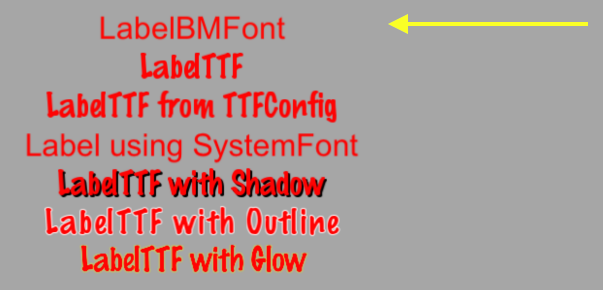
\includegraphics[width=\textwidth]
{figures/label_1}
\end{column}
\end{columns}
\begin{block}{创建BMFont标签}
\begin{verbatim}
auto myLabel = Label::createWithBMFont("bitmapRed.fnt", "Text");
\end{verbatim}
\end{block}
\end{frame}

% Page 61

\begin{frame}[fragile]{标签(Label)}
\begin{columns}
\begin{column}{0.4\textwidth}
TrueType字体和我们上面了解的位图字体不同,使用这种字体很方便,你不需要为每种尺寸和颜色单独使用字体文件。虽然使用TrueType字体比使用位图字体更灵活,但是它渲染速度较慢,并且更改标签的属性(字体,大小)是一项非常消耗性能的操作。
\end{column}
\begin{column}{0.6\textwidth}
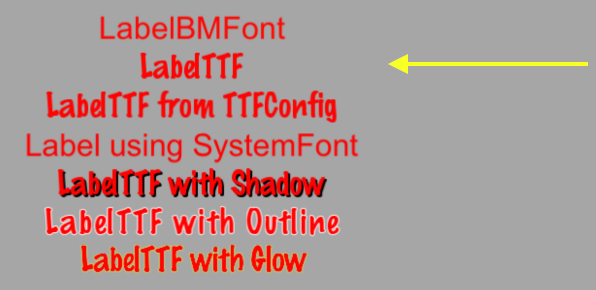
\includegraphics[width=\textwidth]
{figures/label_2}
\end{column}
\end{columns}
\begin{block}{创建TTF标签}
\begin{verbatim}
auto myLabel = Label::createWithTTF("Text", "Marker Felt.ttf", 24);
\end{verbatim}
\end{block}
\end{frame}

% Page 62

\begin{frame}[fragile]{标签(Label)}
如果需要具有相同属性的多个Label对象,那可以创建一个TTFConfig对象来统一配置,TTFConfig对象允许你设置所有标签的共同属性。
\begin{block}{创建TTFConfig对象}
\begin{verbatim}
TTFConfig labelConfig;                         // 创建配置
labelConfig.fontFilePath = "myFont.ttf";       // 字体文件
labelConfig.fontSize = 16;                     // 字体大小
labelConfig.glyphs = GlyphCollection::DYNAMIC; // 使用动态字形
labelConfig.outlineSize = 0;                   // 无外轮廓
labelConfig.customGlyphs = nullptr;            // 无自定义字形
labelConfig.distanceFieldEnabled = false;      // 禁用距离场渲染
// 使用 TTFConfig 配置创建标签
auto myLabel = Label::createWithTTF(labelConfig, "Text");
\end{verbatim}
\end{block}
\end{frame}

% Page 63

\begin{frame}[fragile]{标签(Label)}
\begin{columns}
\begin{column}{0.4\textwidth}
SystemFont是一个使用系统默认字体,默认字体大小的标签类型,这样的标签不要改变他的属性,它会使用系统的规则。
\end{column}
\begin{column}{0.6\textwidth}
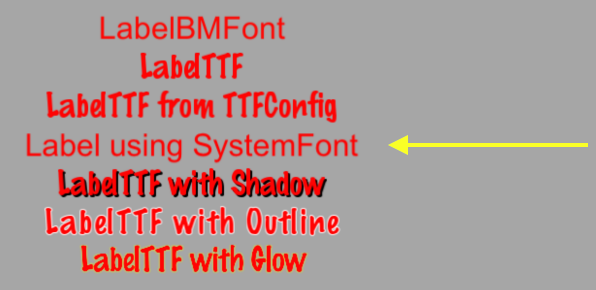
\includegraphics[width=\textwidth]
{figures/label_3}
\end{column}
\end{columns}
\begin{block}{创建SystemFont标签}
\begin{verbatim}
auto myLabel = Label::createWithSystemFont("Text", "Arial", 16);
\end{verbatim}
\end{block}
\end{frame}

% Page 64

\begin{frame}[fragile]{标签(Label)}
\begin{columns}
\begin{column}{0.4\textwidth}
标签可以添加阴影效果。
\end{column}
\begin{column}{0.6\textwidth}
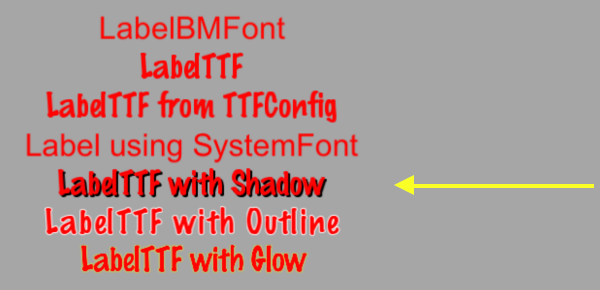
\includegraphics[width=\textwidth]
{figures/label_4}
\end{column}
\end{columns}
\begin{block}{创建阴影效果标签}
\begin{verbatim}
auto myLabel = Label::createWithTTF("myFont.ttf", "Text", 16);
myLabel->enableShadow();
\end{verbatim}
\end{block}
\end{frame}

% Page 65

\begin{frame}[fragile]{标签(Label)}
\begin{columns}
\begin{column}{0.4\textwidth}
标签可以添加描边效果。
\end{column}
\begin{column}{0.6\textwidth}
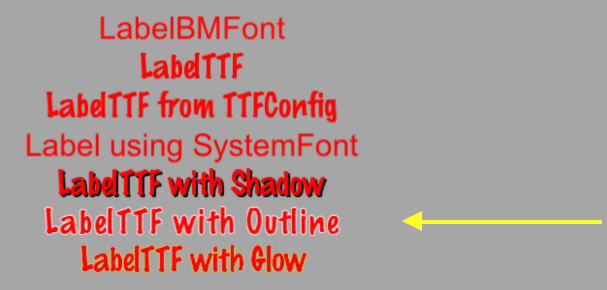
\includegraphics[width=\textwidth]
{figures/label_5}
\end{column}
\end{columns}
\begin{block}{创建描边效果标签}
\begin{verbatim}
auto myLabel = Label::createWithTTF("myFont.ttf", "Text", 16);
myLabel->enableOutline(Color4B::WHITE, 1);
\end{verbatim}
\end{block}
\end{frame}

% Page 66

\begin{frame}[fragile]{标签(Label)}
\begin{columns}
\begin{column}{0.4\textwidth}
标签可以添加发光效果。
\end{column}
\begin{column}{0.6\textwidth}
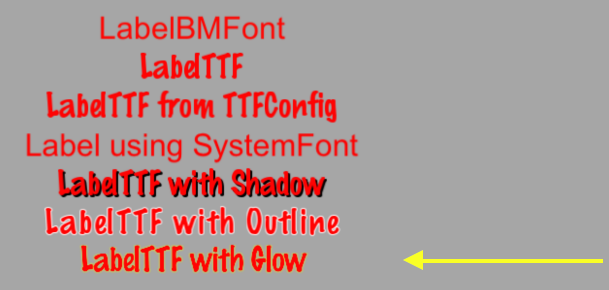
\includegraphics[width=\textwidth]
{figures/label_6}
\end{column}
\end{columns}
\begin{block}{创建发光效果标签}
\begin{verbatim}
auto myLabel = Label::createWithTTF("myFont.ttf", "Text", 16);
myLabel->enableGlow(Color4B::YELLOW);
\end{verbatim}
\end{block}
\end{frame}

% Page 67

\begin{frame}[fragile]{菜单(Menu)}
\begin{block}{创建菜单}
\begin{verbatim}
// 创建一个存储菜单项的 Vector
Vector<MenuItem*> MenuItems;

// 创建一个关闭菜单项,使用图片并绑定回调函数
auto closeItem = MenuItemImage::create("Normal.png", "Selected.png",
    CC_CALLBACK_1(HelloWorld::menuCloseCallback, this));

// 将关闭菜单项添加到 MenuItems 向量中
MenuItems.pushBack(closeItem);

/* 如果有更多的菜单项,可以继续类似地创建并添加到 MenuItems 向量中 */
\end{verbatim}
\end{block}
\end{frame}

% Page 68

\begin{frame}[fragile]{菜单(Menu)}
\begin{block}{创建菜单}
\begin{verbatim}
/* 如果有更多的菜单项,可以继续类似地创建并添加到 MenuItems 向量中 */
auto anotherItem = MenuItemImage::create("Normal.png", "Selected.png",
    CC_CALLBACK_1(HelloWorld::anotherCallback, this));
MenuItems.pushBack(anotherItem);

// 创建菜单,并将 MenuItems 向量传递给它
auto menu = Menu::createWithArray(MenuItems);

// 将菜单添加到当前节点(假设当前节点是 this),设置层级为 1
this->addChild(menu, 1);
\end{verbatim}
\end{block}
\end{frame}

% Page 69

\begin{frame}[fragile]{按钮(Button)}
按钮会拦截点击事件,事件触发时调用事先定义好的回调函数。按钮有一个正常状态,一个选择状态,还有一个不可点击状态,按钮的外观可以根据这三个状态而改变。(\hrefcol{https://github.com/MinmusLin/Teamfight_Tactics/blob/main/Classes/Button}{HoverButton类})

\vspace{1em}

在屏幕显示的时候,同一个时刻只能看到一个状态,正常显示状态像这样:

\vspace{1em}

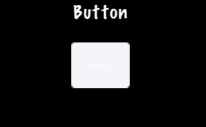
\includegraphics[width=0.3\textwidth]
{figures/button}
\end{frame}

% Page 70

\begin{frame}[fragile]{按钮(Button)}
\begin{block}{创建按钮}
\begin{verbatim}
auto button = Button::create("normal_image.png",
                             "selected_image.png",
                             "disabled_image.png");
button->setTitleText("Button Text");
button->addTouchEventListener([&](Ref* sender,
                                  Widget::TouchEventType type) {
    switch (type) {
        case ui::Widget::TouchEventType::BEGAN: ...
        case ui::Widget::TouchEventType::ENDED: ...
        default: break;
    }
});
\end{verbatim}
\end{block}
\end{frame}

% Page 71

\begin{frame}[fragile]{复选框(CheckBox)}
只有两种状态的项目经常被设计为复选框。我们为一个复选框指定了五张图像,因为复选框有五种状态:未被选中,被点击,未被选中时不可用,被选中,选中时不可用。这样五种状态的图像依次如下:

\vspace{1em}


\includegraphics[width=0.5\textwidth]
{figures/checkbox_status}

\vspace{1em}

在屏幕显示的时候,同一个时刻只能看到一个状态,被选中时状态像这样:

\vspace{1em}

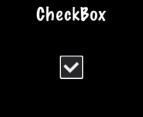
\includegraphics[width=0.2\textwidth]
{figures/checkbox}
\end{frame}

% Page 72

\begin{frame}[fragile]{复选框(CheckBox)}
\begin{block}{创建复选框}
\begin{verbatim}
auto checkbox = CheckBox::create("check_box_normal.png",
    "check_box_normal_press.png", "check_box_active.png",
    "check_box_normal_disable.png", "check_box_active_disable.png");
checkbox->addTouchEventListener([&](Ref* sender,
                                    Widget::TouchEventType type) {
    switch (type) {
        case ui::Widget::TouchEventType::BEGAN: ...
        case ui::Widget::TouchEventType::ENDED: ...
        default: ...
    }
});
\end{verbatim}
\end{block}
\end{frame}

% Page 73

\begin{frame}[fragile]{进度条(LoadingBar)}
进度条当进度增加时,进度条向右填充。在屏幕上一个满进度的进度条是这样的:

\vspace{1em}


\includegraphics[width=0.2\textwidth]
{figures/loading_bar}

\vspace{1em}

\begin{block}{创建进度条}
\begin{verbatim}
auto loadingBar = LoadingBar::create("LoadingBarFile.png");
loadingBar->setDirection(LoadingBar::Direction::RIGHT);

loadingBar->setPercent(25);
loadingBar->setPercent(35);
\end{verbatim}
\end{block}
\end{frame}

% Page 74

\begin{frame}[fragile]{滑动条(Slider)}
实现一个滑动条需要提供五张图像,对应滑动条的不同部分不同状态,分别为:滑动条背景,上层进度条,正常显示时的滑动端点,滑动时的滑动端点,不可用时的滑动端点。

\vspace{1em}


\includegraphics[width=\textwidth]
{figures/slider_status}

\vspace{1em}

在屏幕上一个滑动条看起来是这样的:

\vspace{1em}

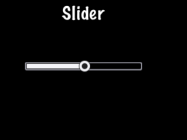
\includegraphics[width=0.2\textwidth]
{figures/slider}
\end{frame}

% Page 75

\begin{frame}[fragile]{滑动条(Slider)}
\begin{block}{创建滑动条}
\begin{verbatim}
auto slider = Slider::create();
slider->loadBarTexture("Slider_Back.png");
slider->loadSlidBallTextures("Normal.png","Press.png","Disable.png");
slider->loadProgressBarTexture("Slider_PressBar.png");
slider->addTouchEventListener([&](Ref* sender,
                                  Widget::TouchEventType type) {
    switch (type) {
        case ui::Widget::TouchEventType::BEGAN: ...
        case ui::Widget::TouchEventType::ENDED: ...
        default: ...
    }
});
\end{verbatim}
\end{block}
\end{frame}

% Page 76

\begin{frame}[fragile]{文本框(TextField)}
\begin{block}{创建滑动条}
\begin{verbatim}
auto slider = Slider::create();
slider->loadBarTexture("Slider_Back.png");
slider->loadSlidBallTextures("Normal.png","Press.png","Disable.png");
slider->loadProgressBarTexture("Slider_PressBar.png");
slider->addTouchEventListener([&](Ref* sender,
                                    Widget::TouchEventType type) {
    switch (type) {
        case ui::Widget::TouchEventType::BEGAN: ...
        case ui::Widget::TouchEventType::ENDED: ...
        default: ...
    }
});
\end{verbatim}
\end{block}
\end{frame}





\backmatter
\end{document}